\section{Efficiency}

The basic design described in the previous section, while functional, would produce
somewhat inefficient instrumented code. 


\subsection{Function Relocation}
The novel use of relocation at the function level in our instrumentation strategy stems from the fact
that we are performing the instrumentation statically on a platform that uses a
variable-length instruction set. A typical strategy used by static
instrumentation tools on platforms with fixed-length instruction sets is to
replace a single fixed-length instruction at the instrumentation point with a
branch instruction that will transfer control to the code produced by the
instrumentation tool. This is fairly straightforward to do because by the
definition of a fixed-length instruction set, the instruction being replaced and
the replacement branch have the same length. Performing static instrumentation
in a variable-length instruction set does not afford us this luxury. In X86, an
unconditional branch that uses a 32-bit offset requires 5 bytes, whereas some of
the instrumentation points that interest us may use only a single byte.

This leaves two options for how to transfer control to the instrumentation code.
We must either use a technique entirely distinct from the idea of using a single
unconditional branch to execute the control transfer such as multiple shorter
jumps or software interrupts, or we must somehow alter the application code so
that it can accomodate a single large control instruction that is larger than
the original amount of space available at the instrumentation point. A seperate
technique for transferring control flow could be to use a series of branches,
where the instruction in the instrumentation point is a small branch that
transfers control to a larger intermediate branch. We do not consider this
method any further because the smallest unconditional branch instruction is 2
bytes in length, making it ultimately a half measure since there are
instrumentation points with only a single byte available to them. Another option
to consider is the method proposed by the BIRD project \ref{nanda2006bird}. They
propose using the single-byte \begin{it}INT 3\end{it} instruction, a single-byte
interrupt intended to be used by debuggers to set breakpoints, when a larger
branch won't fit within the specified area. This instructions is functionally
perfect for static instrumentation because it consumes only a single byte and
allows us to transfer control to an arbitrary location by registering an
exception handler with the system. We performed a cursory study on this scheme
from an efficiency standpoint to determine whether it was worth further
investigation. On a small benchmark set, our implementation of using
\begin{it}INT 3\end{it} only when 5-byte unconditional branches do not fit at
the instrumentation point introduces slowdowns of no less than 100-fold for
counting the number of executions of each basic block in the code. As one might
expect, this mechanism is unsuitable for efficient instrumentation because the
very heavyweight system call conventions are being invoked fairly often.

We use the latter option, reorganizing the code at the function level so that
there is enough space at every instrumentation point to accomodate a 5-byte
branch. Specifically, the steps we use are as follows:
\begin{enumerate}
\item 
1. Function Displacement
\item
2. Link Function Entries 
\item
3. Branch Conversion
\item
4. Instruction Padding
\end{enumerate}


Figure \ref{Figure:Relocation} gives a visual version of this process.
\begin{figure}[ht]
\centering
\caption[Optional caption for list of figures]
{The steps taken in order to prepare a function for instrumentation which collects
the memory addresses of an application.}
\subfigure[The two-segment structure of an unmodified ELF file.]{
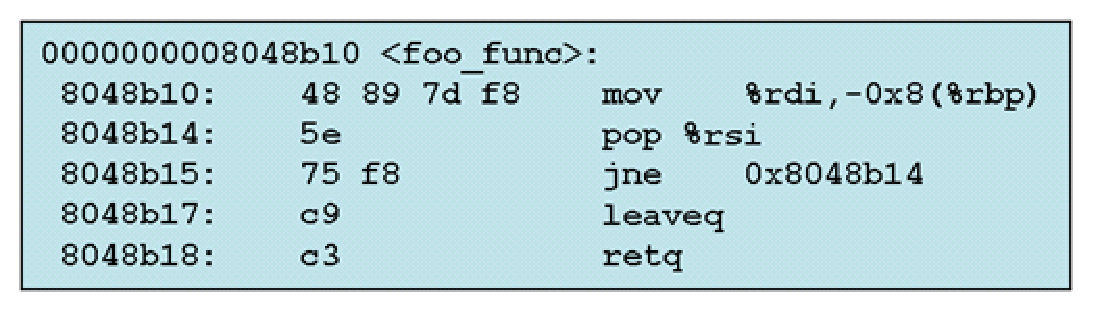
\includegraphics[scale=0.38]{funcp1.eps}
\label{Figure:funcp1}
}
\subfigure[The two-segment structure of an unmodified ELF file.]{
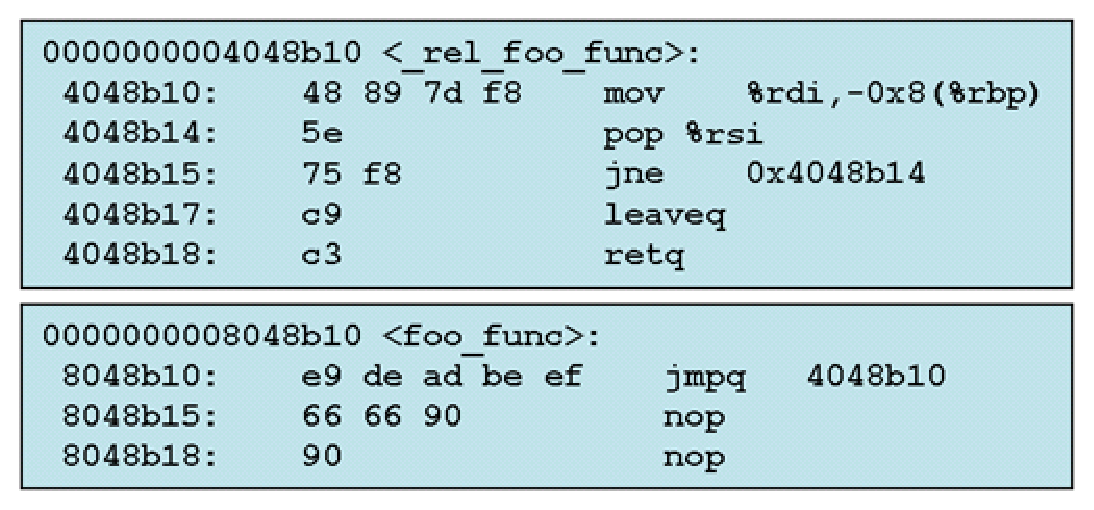
\includegraphics[scale=0.38]{funcp2.eps}
\label{Figure:funcp2}
}
\subfigure[The two-segment structure of an unmodified ELF file.]{
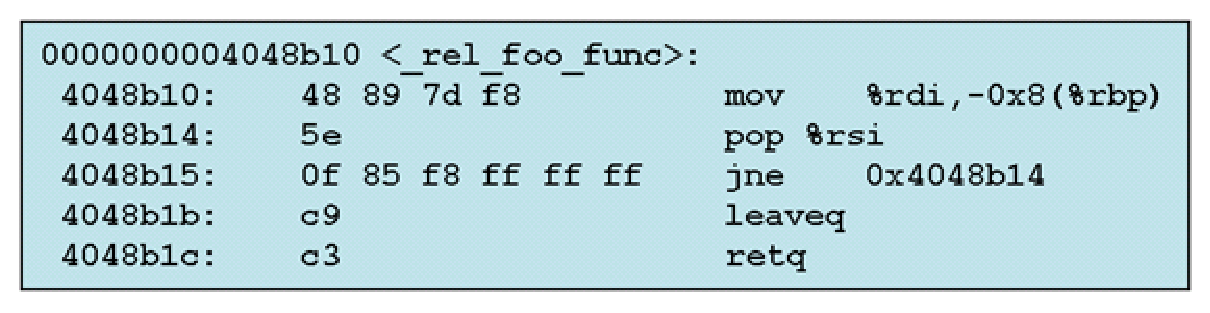
\includegraphics[scale=0.34]{funcp3.eps}
\label{Figure:funcp3}
}
\subfigure[The two-segment structure of an unmodified ELF file.]{
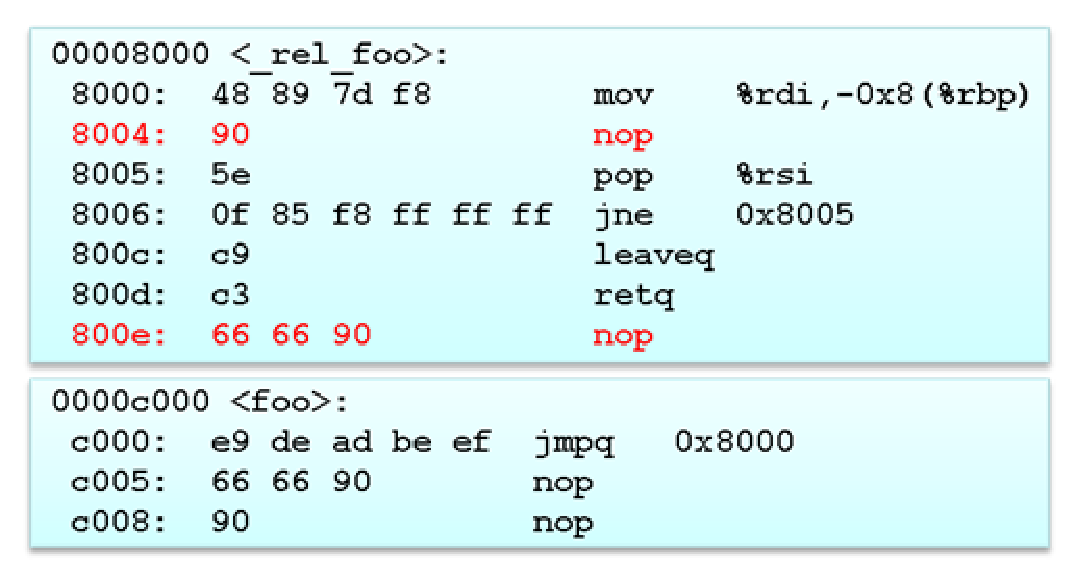
\includegraphics[scale=0.34]{funcp4.eps}
\label{Figure:funcp4}
}
\subfigure[The two-segment structure of an unmodified ELF file.]{
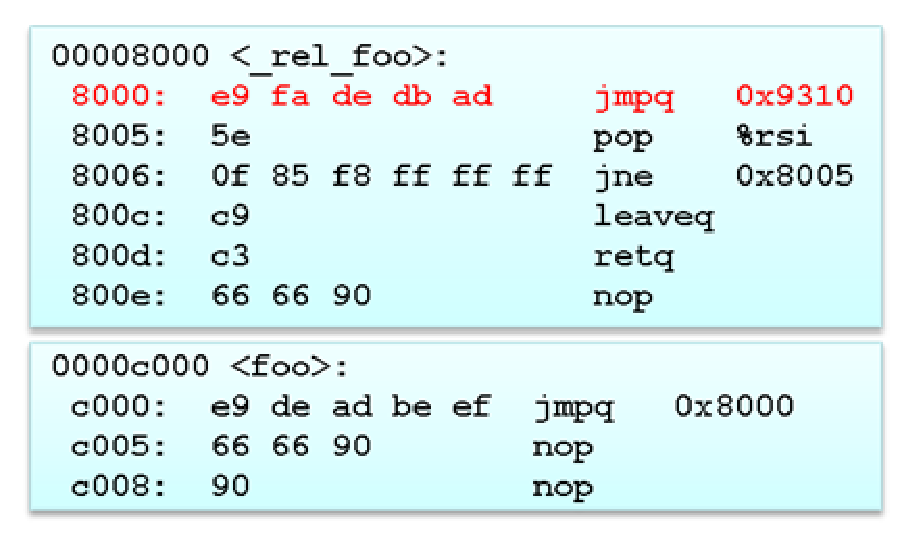
\includegraphics[scale=0.34]{funcp5.eps}
\label{Figure:funcp5}
}
\label{Figure:Relocation}
\end{figure}


1. Function Displacement: Relocate the contents of the entire function to an area of the text section allocated
to the instrumentation tool. Since functions are often packed tightly together, it is generally not possible to
expand the size of a function without disturbing the entry points of another function.

2. Link Function Entries: Place an unconditional branch at the former function entry point that transfers control
to the new function entry point. Most references to the entry point of a function are in the form of function calls, which
routinely are indirect references (ie their value is computed or looked up at runtime) and are difficult to resolve
prior to runtime.

3. Branch Conversion: Convert each short conditional branch in the relocated function to the equivalent
5-byte branch instruction. Since the code is being reorganized in the next step which may strain the limits of
smaller 8-bit or 16-bit offsets, we convert all branches to use 32-bit offsets so that the targets of each branch
will still be reachable without having the need to further reorganize the code. Note that there is some opportunity
here to reduce space by using the smallest branch offset size that accomodates the branch, but this is an issue
for future work.

4. Instruction Padding: According to the needs of the instrumentation tool, pad the instruction at each instrumentation
point with \begin{it}nop\end{it} instructions so that a 5-byte branch can fit.

There are several ways that this process can adversely affect the performance of the application independant of the overhead
that will be imposed by inserting any extra instrumentation code. Each function call
now has an extra control interruption associated with it since control must be passed first to the original function entry
point and then to the relocated function entry point. It is possible that using 32-bit offsets for every branch rather than
some smaller number of bits has an overhead associated with it. And since the code is being reorganized and expanded, 
we might destroy some positive alignment and size optimizations that the compiler might have made on the instructions in the
function. We examine the practical overhead seen by these techniques by taking these steps without instrumenting the code
for a series of benchmarks. The slowdown is XXXX...

\subsection{Disassembly Coverage}
Code and data can reside together in the text section of a program binary. This is done for a variety of reasons, including
the storage of branch target locations (eg for a jump table) or small data structures that provide convenient lookup
of certain data such as identifiers, descriptors, or other values.

Correctly determining
what parts of the text sections are code and what are data is important. Consider what can happen
if we mistakenly treat some data as code. We might choose to modify or relocate the apparent code
to serve our instrumentation purposes. Then when the data at this location is referenced, the
original program behavior may not be preserved: if we are lucky this will cause application failure
due to some unexpected change in control flow or some state condition that is checked by the program.
If we are unlucky the corruption might silently manifest itsself by modifying the output of the
program. Alternatively consider what can happen if we mistakenly treat some code as data. We then will
not try to insert code into this area or we might perform some other type of analysis that should be reserved for
data alone. While this is almost certainly preferrable to the situation where we treat data as code, it
is ideal to avoid both situations.

To this end, we use the program's symbol table to help us determine which parts of the text sections
are functions that are eligible to be subject for our code discovery algorithm. Our code discovery algorithm
consists of two phases; control-driven disassembly backed up by linear disassembly. In more detail, the algorithm
works as follows:

\begin{enumerate}
\item 
1. Control-driven disassembly: from a function's entry point, follow all understandable control paths. If a problem is encountered, fall back to
naive disassembly.
\item
2. Naive disassembly: from a function's entry point, disassemble each instruction in the order it appears in the
function. If a problem is encountered, give up.
\end{enumerate}


Problems that can be encountered are situations where an unknown opcode is encountered, where control jumps to the
middle of an instruction we've already disassembled, or if control leaves the boundaries of the function. In most
cases control-driven disassembly is sufficient to disassemble the entirety of a function, and in most cases control-driven
disassembly is a straightforward process because control either falls through to the following instruction 
or the location of a branch target is embedded entirely within the instruction itsself. But there are also cases
where the an indirect branch is used, where the target resides either at a fixed address (possibly with some offset), the address that resides in a register,
or the address that is at a location given by a register. The latter two cases are very difficult to resolve
without runtime information because the computation of the target address can be arbitrarily complex and can span function
boundaries. Nevertheless, we perform a peephole examination of the previous instructions to the and can determine 
the address in simple cases.

Fortunately simple calculations are all that most compilers use to determine targets for jump tables, one of the more common
uses of an indirect branch. Often an offset is added to a fixed location to determine where the data comprising the branch target
resides. Therefore we treat such a fixed address as the first entry in a table whose entries are treated either as addresses or as offsets.
We then make an iterative pass over this table to determine the target for each arm of the jump table, stopping when we find a value in the
table that yeilds an address that is outside the scope of the function.

PUT EXAMPLE OF GNU COMPILER JUMP TABLE HERE

\subsection{Instrumentation Snippets}
